\chapter{矩阵运算\ 矩阵的秩}

\section{Overview}
\begin{figure}[h]
	\centering
	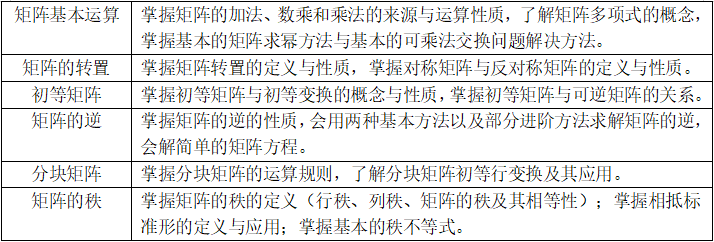
\includegraphics[scale=0.58]{4.png}
\end{figure}

\section{矩阵基本运算}
\subsection{基本概念}
\begin{enumerate}
	\item 矩阵的加法来源于线性映射的加法,矩阵相加要求两矩阵行列数一致,相加时只需对应位置元素相加即可;
	\item 矩阵的数乘来源于线性映射的数乘,计算只需矩阵的每个元素乘以常数即可;
	\item 矩阵的乘法来源于线性映射的复合,计算时要求前一个矩阵的列数等于后一个矩阵的行数,矩阵$A$与$B$
	相乘结果中第$i$行第$j$列元素为矩阵$A$的第$i$行与矩阵$B$的第$j$列对应位置元素相乘后求和的结果,
	即对于$A=(a_{ij})_{m \times n}$和$B=(b_{ij})_{n \times l}$,矩阵$C=AB=(c_{ij})_{m \times l}$,且
	$c_{ij}=a_{i1}b_{1j}+a_{i2}b_{2j}+\cdots+a_{in}b_{nj},\ i=1,\cdots,m,j=1,\cdots,l$.
\end{enumerate}

\subsection{基本性质}
\begin{enumerate}
	\item 回顾上一专题中$m \times n$矩阵构成的线性空间$M_{m \times n}(\mathbf{F})$;
	\item 回顾矩阵乘法的基本性质:
	\begin{enumerate}
		\item $(AB)C=A(BC)$(结合律)
		\item $\lambda(AB)=(\lambda A)B=A(\lambda B)$(其中$\lambda$是数量)
		\item $A(B+C)=AB+AC$(左分配律)
		\item $(B+C)P=BP+CP$(右分配律)
		\item $A^kA^m=A^{k+m}$,$(A^k)^m=A^{km}$,其中$A$为方阵,$k$,$m$为任意整数,
		负整数对应于逆矩阵的情况。
	\end{enumerate}
	\item 回顾矩阵多项式的定义(利用线性映射多项式在基下的矩阵表示定义),
	并注意其交换性以及可因式分解性。
\end{enumerate}
\begin{example}
	展开矩阵多项式$(A+\lambda E)^n$.
\end{example}
\begin{example}
	设$f(x),\ g(x) \in \mathbf{F}[x]$,$A,\ B \in M_n(\mathbf{F})$,证明:
	$$f(A)g(A)=g(A)f(A);$$
	
	\textup{1. }如果$AB=BA$,则$f(A)g(B)=g(B)f(A)$\textup{;}

	\textup{2. }设$f(x)=1+x+\cdots+x^{m-1}$,$g(x)=1-x$,$A=\begin{pmatrix}
		a & b \\ 0 & a
	\end{pmatrix}$,计算$f(A)g(A)$.
\end{example}
其他需要注意的性质:
\begin{enumerate}
	\item 矩阵乘法不一定满足交换律(即$AB$不一定等于$BA$)。但是注意数量矩阵和任何矩阵相乘都是可交换的,因此求矩阵的幂次时,可以将其转化为$(A+\mu E)^n$(其中$E$为单位矩阵,$\mu$为常数)类型,然后利用二项式展开即可。很多情况下$A$都会是幂零矩阵,此时结果为有限项。
	\item $A\neq O$且$B\neq O$不能推出$AB\neq O$。例如线性方程组$AX = 0$有非零解,若$B$的各列均为方程非零解,则$AB = O$。
	\item 消去律也不一定满足:即$AC = BC$不一定$B = C$。原因在于$AB=AC \to A(B-C)=O$,由(2)可知不一定$B = C$。
\end{enumerate}

\subsection{矩阵可交换问题}
一般来说在本课程中此类问题直接设可交换矩阵的每一个元素都是未知数即可,一些特殊的技巧
(使用关于一些特殊形状矩阵的结论)以及涉及到之后才能学到的知识的方法我们在这里也不展开了。我们只讨论一个基本的技巧,即
$$\forall t,\ AB=BA \iff (A-tE)B=B(A-tE)$$
此处的$t$根据矩阵的对角线上元素来决定,原则是使得其余矩阵与$A-tE$相乘的计算过程更为简单(一般是使得0元素更多),这样解方程也会更轻松。
我们来看一个简单的例子:
\begin{example}
	求与矩阵$A=\begin{pmatrix}
		3 & 0 & 0 \\ -1 & 3 & 0 \\ 0 & -1 & 3
	\end{pmatrix}$可交换的矩阵.
\end{example}

关于可交换我们有以下定理,证明并不是很复杂(教材习题中有出现):
\begin{theorem}
	\textup{(1)}与主对角元两两互异的对角矩阵可交换的方阵只能是对角矩阵;

	\textup{(2)}准对角矩阵$A$每个对角分块内对角线元素相同,但不同对角块之间不同,则与$A$可交换的矩阵只能是准对角矩阵;
	
	\textup{(3)}与所有$n$级可逆矩阵可交换的矩阵为数量矩阵;
	
	\textup{(4)}与所有$n$级矩阵可交换的矩阵为数量矩阵.
\end{theorem}


\subsection{习题}
\centerline{\heiti A组}
\begin{enumerate}
	\item 证明:若$AB=BA$,$AC=CA$,则$A,\ B,\ C$为同阶方阵,且
	$$A(BC)=(BC)A,\ A(B+C)=(B+C)A.$$
	\item $A,\ B$都是$n$阶矩阵,求下列等式成立的充分条件:
	
	(1)$(A+B)^3=A^3+3A^2B+3AB^2+B^3$;

	(2)$(A+B)(A-B)=A^2-B^2$.
\end{enumerate}
\centerline{\heiti B组}
\begin{enumerate}
	\item 已知矩阵$A=\begin{pmatrix}
		1 & 0 & 4 \\ 0 & 1 & 2 \\ 0 & 1 & 2
	\end{pmatrix}$,求证:所有与$A$可交换的矩阵构成$M_3(\mathbf{R})$的一个子空间,并求子空间的一组基.
	\item 若$f(x)$是$x$的实系数$m$次多项式:
	$$f(x)=a_mx^m+a_{m-1}x^{m-1}+\cdots+a_1x+a_0,$$
	则有矩阵多项式:
	$$f(A)=a_mA^m+a_{m-1}A^{m-1}+\cdots+a_1A+a_0E\ (A^0=E).$$

	(1)若$A$为对角矩阵$B=\begin{pmatrix}
		\lambda_1 & 0 \\ 0 & \lambda_2
	\end{pmatrix}$,证明:$f(A)=\begin{pmatrix}
		f(\lambda_1) & 0 \\ 0 & f(\lambda_2)
	\end{pmatrix}$;

	(2)若$A=P^{-1}BP$,证明:$f(A)=P^{-1}f(B)P$.
\end{enumerate}

\centerline{\heiti C组}
\begin{enumerate}
	\item 证明以下两个命题:
	
	(1)与矩阵$I=\begin{pmatrix}
		0 & 1 & 0 & \cdots & 0 & 0 \\
		0 & 0 & 1 & \cdots & 0 & 0 \\
		0 & 0 & 0 & \cdots & 0 & 0 \\
		\vdots & \vdots & \vdots &  & \vdots & \vdots \\
		0 & 0 & 0 & \cdots & 0 & 1 \\
		1 & 0 & 0 & \cdots & 0 & 0
	\end{pmatrix}$可交换的矩阵$A$都可以写成$I$的一个多项式,即
	$A=a_{11}E+a_{12}I+a_{13}I^2+\cdots+a_{1n}I^{n-1}$;
	
	(2)与矩阵$J=\begin{pmatrix}
		0 & 1 & 0 & \cdots & 0 & 0 \\
		0 & 0 & 1 & \cdots & 0 & 0 \\
		0 & 0 & 0 & \cdots & 0 & 0 \\
		\vdots & \vdots & \vdots &  & \vdots & \vdots \\
		0 & 0 & 0 & \cdots & 0 & 1 \\
		0 & 0 & 0 & \cdots & 0 & 0
	\end{pmatrix}$可交换的矩阵$A$都可以写成$J$的一个多项式,即
	$A=a_{11}E+a_{12}J+a_{13}J^2+\cdots+a_{1n}J^{n-1}$;
\end{enumerate}

\section{矩阵的转置}
\subsection{基本概念}
实际上,矩阵的转置就是第$i$行变成了第$i$列,或者抽象表达为:
$$A=(a_{ij})_{m \times n},\ A^\mathrm{T}=(a'_{ji})_{n \times m},\ a_{ij}=a'_{ji}$$
写成矩阵形式为:
\begin{definition}
	设$A=\begin{pmatrix}
		a_{11} & a_{12} & \cdots & a_{1n} \\
		a_{21} & a_{22} & \cdots & a_{2n} \\
		\vdots & \vdots &       & \vdots \\
		a_{m1} & a_{m2} & \cdots & a_{mn}
	\end{pmatrix}$,称$\begin{pmatrix}
		a_{11} & a_{21} & \cdots & a_{m1} \\
		a_{12} & a_{22} & \cdots & a_{m2} \\
		\vdots & \vdots &       & \vdots \\
		a_{1n} & a_{2n} & \cdots & a_{mn}
	\end{pmatrix}$为矩阵$A$的转置,记作$A^\mathrm{T}$.
\end{definition}

\subsection{基本性质}
1. $(A^\mathrm{T})^\mathrm{T}=A$

2. $(A+B)^\mathrm{T}=A^\mathrm{T}+B^\mathrm{T}$

3. $(\lambda A)^\mathrm{T}=\lambda A^\mathrm{T}$($\lambda$是数量)

4. $(AB)^\mathrm{T}=B^\mathrm{T}A^\mathrm{T}$,$(A_1A_2\cdots A_n)^\mathrm{T}=A_n^\mathrm{T}\cdots A_2^\mathrm{T}A_1^\mathrm{T}$

5. $(A^\mathrm{T})^{-1}=(A^{-1})^\mathrm{T}$

6. $(A^\mathrm{T})^m=(A^m)^\mathrm{T}$

以上证明大都是平凡的,可以自己尝试完成。
\subsection{对阵矩阵与反对称矩阵}
\begin{definition}
	设$A=(a_{ij})_{n \times n}$,如果$\forall i,j=1,2,\cdots$均有$a_{ij}=a_{ji}$,
	则称$A$为对称矩阵,若均有$a_{ij}=-a_{ji}$,则称$A$为反对称矩阵.
\end{definition}
易得$A$为对称矩阵的充要条件为$A=A^\mathrm{T}$,$A$为反对称矩阵的充要条件为$A=-A^\mathrm{T}$.
\begin{example}
	证明以下几点性质:
	
	\textup{1. }反对称矩阵主对角元均为$0$\textup{;}
	
	\textup{2. }$AA^\mathrm{T}$和$A^\mathrm{T}A$均为对称矩阵\textup{;}
	
	\textup{3. }设$A,\ B$为$n$阶对称和反对称矩阵,则$AB+BA$是反对称矩阵\textup{;}
	
	\textup{4. }对称矩阵的乘积不一定对称\textup{;}
	
	\textup{5. }可逆的对称(反对称)矩阵的逆矩阵也是对称(反对称)矩阵。
\end{example}

\subsection{习题}
\centerline{\heiti A组}
\begin{enumerate}
	\item 设$\alpha=(1,-1,2)^\mathrm{T},\ \beta=(2,1,1)^\mathrm{T},\ A=\alpha\beta^\mathrm{T}$,求$A^n$.
	\item 设$\alpha,\ \beta$为三维列向量,且$\alpha\beta^\mathrm{T}=
	\begin{pmatrix}-1 & 2 & 1 \\ 1 & -2 & -1 \\ 2 & -4 & -2\end{pmatrix}
	$,求$\alpha^\mathrm{T}\beta$.
\end{enumerate}
\centerline{\heiti B组}
\begin{enumerate}
	\item 设$A$为$n$阶实矩阵,且$A^\mathrm{T}A=O$,证明:$A=O$.
	\item 设 $V=\{(a_{ij})_{n \times n}\ |\ \forall i,\ j,\ a_{ij}=a_{ji}\}$
	
	(1)证明:$V$ 为 $F^{n \times n}$ 的子空间;
	
	(2)求  $V$ 的基和维数.
	\item 求矩阵$\begin{pmatrix}
		a & b & c & d \\ -b & a & d & -c \\ -c & -d & a & b \\ -d & c & -b & a
	\end{pmatrix}$的逆.
\end{enumerate}

\centerline{\heiti C组}
\begin{enumerate}
	\item $a,b,c,d$是四个实数,证明:$\begin{cases}
		a^2+b^2=1 \\ c^2+d^2=1 \\ ac+bd=0
	\end{cases}$成立的充分必要条件是$\begin{cases}
		a^2+c^2=1 \\ b^2+d^2=1 \\ ab+cd=0
	\end{cases}$.
\end{enumerate}

\section{初等矩阵}
\subsection{基本概念与性质}
\begin{definition}
	将单位矩阵$E$做一次初等变换得到的矩阵称为初等矩阵,与三种初等行、列变换对应的三类初等矩阵为:
	
	\textup{(1)}将单位矩阵第$i$行(或列)乘$c$,得到初等倍乘矩阵$E_i(c)$\textup{;}

	\textup{(2)}将单位矩阵第$i$行乘$c$加到第$j$行,或将第$j$列乘$c$加到第$i$列,得到初等倍加矩阵$E_{ij}(c)$\textup{;}

	\textup{(3)}将单位矩阵第$i,j$行(或列)对换,得到初等对换矩阵$E_{ij}$.
\end{definition}
请各位同学以矩阵形式写出以上三类矩阵。注意:

1. 倍加变化请一定注意$i$和$j$在行列的情况下的不同;

2. 三类矩阵不是三个矩阵,例如行列选择不唯一,常数选择不唯一;

3. 注意三种初等矩阵都是可逆的,且$E_i^{-1}(c)=E_i(\cfrac{1}{c})$,$E_{ij}^{-1}(c)=E_{ij}(-c)$,$E_{ij}^{-1}=E_{ij}$;

4. 三种初等矩阵的转置:$E_i^\mathrm{T}(c)=E_i(c)$,$E_{ij}^\mathrm{T}(c)=E_{ji}(c)$,$E_{ij}^\mathrm{T}=E_{ij}$;

初等矩阵大家非常关心为什么左乘代表行变换,右乘代表列变换。以右乘为例,我们来看矩阵$A$和$B$相乘的任一列结果。我们可以将矩阵$A$
按列做分块矩阵得到$(\alpha_1,\cdots,\alpha_n)$,$\alpha_i$即表示$A$的第$i$列。然后矩阵$B$的第$j$列为列向量$(x_1,\cdots,x_n)^\mathrm{T}$,
由于矩阵$A$与$B$相乘结果第$j$列就是$A$与$B$的第$j$列相乘结果(回顾矩阵乘法的计算方式),则有$B$的第$i$列等于
$x_1\alpha_1+\cdots+x_n\alpha_n$即为$A$的全部列向量的线性组合,故右乘矩阵$A$得到矩阵的任一列都是$A$的全部列向量的线性组合,
所以右乘可以代表列变换。注意我这里并没有限制矩阵$B$为初等矩阵或可逆矩阵。

实际上左乘表示行变换可以用类似方法说明,只需按行对$B$分块即可。这一思想是特别重要的,在很多时候如果我们意识到左右乘是对被乘矩阵的行列
重新线性组合,思路会清晰很多。

关于初等矩阵还有一个相当重要的定理:
\begin{theorem}
	任意可逆矩阵都可以被表示为若干个初等矩阵的乘积.
\end{theorem}
定理证明只需要回忆高斯消元法可以将可逆矩阵化为单位矩阵即可。

利用矩阵初等变换我们可以获得本学期需要学习的三个矩阵标准形,因此这一内容虽然很基本但是非常重要:
\begin{enumerate}
	\item 相抵矩阵:本章已学习的内容,在之后会详细说明;
	\item 相似矩阵:若$P$为初等矩阵,对矩阵做$P^{-1}AP$变换即可得到与$A$相似的矩阵;
	\item 相合矩阵:两个矩阵,其中一个可以通过做相同的初等行列变换的到另一个矩阵(若$P$为初等矩阵,
	$P^{\mathrm{T}}AP$就是对$A$做了一次相同的初等行列变换)。
\end{enumerate}
请同学们思考:如何从线性映射矩阵表示的角度理解初等变换与标准形的关系?在B组习题中将有练习进行体会
(实际上对矩阵表示的基做“初等变换”就是对表示矩阵做了初等变换,这两种变换行列方向不一致且矩阵互逆)。

\subsection{习题}
\centerline{\heiti A组}
\begin{enumerate}
	\item 设$A$为三阶矩阵,将A的第二列加到第一列得到矩阵$B$,再对调$B$的$2$、$3$行得到单位矩阵,
	令$P_1=\begin{pmatrix}1 & 0 & 0 \\ 1 & 1 & 0 \\ 0 & 0 & 1\end{pmatrix}$,
	$P_2=\begin{pmatrix}1 & 0 & 0 \\ 0 & 0 & 1 \\ 0 & 1 & 0\end{pmatrix}$,试用
	$P_1$和$P_2$表示$A$.
	\item 设$A$为可逆矩阵,将$A$的第$i$行和第$j$行对调得到矩阵$B$,证明矩阵$B$可逆并求$AB^{-1}$.
	\item 设$A$为三阶可逆矩阵,且$P^{-1}AP=\begin{pmatrix}1 & 0 & 0 \\ 0 & 1 & 0 \\ 0 & 0 & 2\end{pmatrix}$,
	其中$P=(\alpha_1,\alpha_2,\alpha_3)$,令$Q=(\alpha_1+\alpha_2,\alpha_2,\alpha_3)$,求$Q^{-1}AQ$.
\end{enumerate}
\centerline{\heiti B组}
\begin{enumerate}
	\item 已知$\mathbf{R}^3$的基$B_1=\{\alpha_1,\alpha_2,\alpha_3\}$变为基$B_2=\{\xi_1,\xi_2,\xi_3\}$的变换矩阵
	为$A=(a_{ij})_{3 \times 3}$,求:

	(1)基$B_3=\{\alpha_2,\alpha_1,\alpha_3\}$变为基$B_2$的变换矩阵;

	(2)基$B_4=\{-\alpha_1,\alpha_2,\alpha_3\}$变为基$B_2$的变换矩阵;

	(3)基$B_4$变为基$B_5=\{\xi_3,\xi_2,-\xi_1\}$的变换矩阵;

	(4)基$B_4$变为基$B_6=\{\xi_1+\xi_2,\xi_2+\xi_3,\xi_3+\xi_1\}$的变换矩阵.
	\item 设$P=\begin{pmatrix}
		1 & 1 & 0 \\ 0 & 1 & 0 \\ 0 & 0 & 0
	\end{pmatrix}$,$Q=\begin{pmatrix}
		0 & 0 \\ 1 & 0
	\end{pmatrix}$,定义$\mathbf{R}^{3\times 2}$上映射$\sigma(A)=PAQ$,

	(1)验证$\sigma$是线性映射;

	(2)求$\ker\sigma$和$\textup{Im }\sigma$;

	(3)求$\mathbf{R}^{3\times 2}$的两组基,使得$\sigma$关于这两组基的表示矩阵是对角矩阵.
\end{enumerate}

\section{可逆矩阵}
\subsection{基本概念}
\begin{definition}
	设$A \in M_n(\mathbf{F})$,如果存在$B \in M_n(\mathbf{F})$,使得$AB=BA=E$则称矩阵$A$可逆,
	并把$B$称为$A$的逆矩阵.
\end{definition}
注意,逆矩阵定义基于方阵,非方阵没有上述逆矩阵。广义逆矩阵允许非方阵,但那是另一个定义,
我们不需要掌握。对于可逆矩阵,注意以下两个定理:
\begin{theorem}
	可逆矩阵$A$的逆矩阵唯一.
\end{theorem}
\begin{theorem}
	$AB=E \iff A$与$B$互为逆矩阵.
\end{theorem}
这两个定理的证明教材中有,特别注意唯一性的证明,反证法的思路一定要掌握,十分经典。
还需要强调的一点是,逆矩阵来源于逆映射。
\subsection{基本性质}
1. 注意没有加法性质(请举出反例),对于数乘有$(\lambda A)^{-1}=\lambda^{-1}A^{-1}$;

2. $(AB)^{-1}=B^{-1}A^{-1}$,$(A_1A_2\cdots A_k)^{-1}=A_k^{-1}\cdots A_2^{-1}A_1^{-1}$;

3. $(A^k)^{-1}=(A^{-1})^k$,$A^kA^m=A^{k+m}$,$(A^k)^m=A^{km}$;

4. 若$A$和$B$可逆,则$A\neq O$且$B\neq O$能推出$AB\neq O$,并且$A$可逆且$AB=O$可以推出$B=O$,
除此之外还有消去律成立,即$A$则有$AB=AC \Rightarrow B=C$成立.

还需要熟练掌握可逆矩阵的几个等价条件:
\begin{theorem}
	设$A \in M_n{\mathbf{F}}$,则下列命题等价:

	\textup{(1)}$A$可逆;
	
	\textup{(2)}$r(A)=n$;
	
	\textup{(3)}$A$的$n$个行(列)向量线性无关;
	
	\textup{(4)}齐次线性方程组$AX=0$只有零解;
	
	\textup{(5)}$|A|\neq 0$.
\end{theorem}
\begin{example}
	已知矩阵 $A=\begin{pmatrix}a & b & c \\ d & e & f \\ h & x & y\end{pmatrix}$ 的逆是 $A^{-1}=\begin{pmatrix}-1 & -2 & -1 \\ 2 & 1 & 0 \\ 0 & -3 & -1\end{pmatrix}$,

$B=\begin{pmatrix}a-2b & b-3c & -c \\ d-2e & e-3f & -f \\ h-2x & x-3y & -y\end{pmatrix}$。求矩阵 $X$ 满足:

$$X+(B(A^TB^2)^{-1}A^T)^{-1}=X(A^2(B^TA)^{-1}B^T)^{-1}(A+B)$$
\end{example}

\subsection{逆矩阵的求解(基本方法)}
1. 利用解线性方程组的方法:假设$AX=b$,使用高斯消元法求解;

2. 利用初等矩阵的方法(初等行变换为常用方法)。

注意,基于初等变换的方法是非常重要的,我们很多时候不要被题目吓到去采用其他
偏门的方法,实际上很多时候拿到一个具体的矩阵求逆,使用的方法就是初等行变换。

\begin{example}
	用上述两种方法求矩阵$A=\begin{pmatrix}1 & -1 & 1 \\ 0 & 1 & 2 \\ 1 & 0 & 4\end{pmatrix}$的逆矩阵.
\end{example}
\subsection{矩阵方程}
\begin{enumerate}
	\item 考虑以下情形(其中出现的矩阵除$X$外均可逆,$X$不一定是列向量):
	\begin{enumerate}
		\item $AX=B \Rightarrow X=A^{-1}B$,$XA=B \Rightarrow X=BA^{-1}$;
		\item $AXB=C \Rightarrow X=A^{-1}CB^{-1}$;
	\end{enumerate}
	\item 考虑以下情形:$AX=B$但$A$不可逆($X$不一定是列向量),直接高斯消元即可;
	\item 考虑以下求解方式的合理性:
	\begin{enumerate}
		\item 若求$A^{-1}$,只需对$(A,E)$只做初等行变换,可以得到$(E,A^{-1})$;
		\item 若求$A^{-1}B$,只需对$(A,B)$只做初等行变换,可以得到$(E,A^{-1}B)$;
		\item 若求$BA^{-1}$,只需对$\begin{pmatrix}
			A \\ B
		\end{pmatrix}$只做初等列变换,可以得到$\begin{pmatrix}
			E \\ BA^{-1}
		\end{pmatrix}$;
		\item 对$\begin{pmatrix}
			A & E \\ E & O
		\end{pmatrix}$的前$n$行与$n$列做相同的行列变换,可以得到$\begin{pmatrix}
			P^\mathrm{T}AP & P^\mathrm{T} \\ P & O
		\end{pmatrix}$.
	\end{enumerate}
\end{enumerate}

\begin{example}
	设$A=\begin{pmatrix}1 & 0 & 0 \\ 1 & 1 & 0 \\ 1 & 1 & 1\end{pmatrix},\ 
	B=\begin{pmatrix}0 & 1 & 1 \\ 1 & 0 & 1 \\ 1 & 1 & 0\end{pmatrix}$,求矩阵$X$满足:	
	$$AXA+BXB=AXB+BXA+A(A-B)$$
\end{example}

\subsection{习题}
\centerline{\heiti A组}
\begin{enumerate}
	\item 设方阵$A$满足$A^2-A-2E=0$,证明:
	
	(1)$A$和$E-A$都是可逆矩阵,并求它们的逆矩阵;

	(2)$A+E$和$A-2E$不可能同时可逆.
\end{enumerate}

\centerline{\heiti B组}
\begin{enumerate}
	\item 已知矩阵$A=\begin{pmatrix}
		1 & 0 & 1 \\ 0 & 2 & 0 \\ 1 & 0 & 1
	\end{pmatrix}$,
	
	(1)求所有与$A$可交换的矩阵;

	(2)若$AB+E=A^2+B$,求$B$.
	\item 设$A$为$n$阶可逆矩阵,$A$的每行各元素之和都等于$k$,证明:$k \neq 0$且
	$A^{-1}$的每行各元素之和都等于$\cfrac{1}{k}$.
	\item 已知矩阵$A=\begin{pmatrix}1 & 2 & a \\ 1 & 3 & 0 \\ 2 & 7 & -a\end{pmatrix}$可以
	通过初等列变换转化为矩阵$B=\begin{pmatrix}1 & a & 2 \\ 0 & 1 & 1 \\ -1 & 1 & 1\end{pmatrix}$.

	\textup{(1)}求常数$a$;

	\textup{(2)}求满足$AP=B$的可逆矩阵$P$.
\end{enumerate}
\centerline{\heiti C组}
\begin{enumerate}
	\item 设 $A,\ B,\ C$ 为二阶复方阵,且 $A,\ B,\ C$ 在 $M_2(\mathbf{C})$ 中线性无关。证明:存在复数 $x_1,\ x_2,\ x_3$ 使得 $x_1A+x_2B+x_3C$ 为可逆矩阵.
\end{enumerate}
\section{分块矩阵}
注意:从本节起内容难度有所提升,可以根据内容重要程度及自身实际选择性掌握。
\subsection{运算性质}
\begin{definition}
	一般的,对于$m \times n$矩阵$A$,如果在行的方向分成$s$块,在列的方向分成$t$
	块,就得到$A$的一个$s \times t$分块矩阵,记作$A=(A_{kl})_{s \times t}$,其中
	$A_{kl}(k=1,\cdots,s;l=1,\cdots,t)$称为$A$的子块.
\end{definition}
实际上上述表示方法就是将一般矩阵表示$A=(a_{ij})_{m \times n}$中的$a_{ij}$替换为了小块矩阵,
字母含义并无变化,内层代表索引,外层代表总行列数(只是分块矩阵是块索引和块数)。
我们接下来考察分块矩阵的运算性质。

1. 分块矩阵的加法:设分块矩阵$A=(A_{kl})_{s \times t}$,$B=(B_{kl})_{s \times t}$,如果$A$与$B$
对应的子块$A_{kl}$和$B_{kl}$都是同型矩阵,则$$A+B=(A_{kl}+B_{kl})_{s \times t}.$$
由此我们看到分块矩阵加法要求小块形状和行列分块数都一致,实际上回顾一般矩阵加法要求矩阵完全同型即可理解这一要求.

2. 分块矩阵的数乘:设分块矩阵$A=(A_{kl})_{s \times t}$,$\lambda$是一个数,则
$$\lambda A=(\lambda A_{kl})_{s \times t}.$$
实际上数乘最好理解,因为如此计算的效果相当于一般矩阵数乘的效果,即给每个元素
都乘以一个常数$\lambda$.

3. 分块矩阵的乘法:设$A=(a_{ij})_{m \times n}$,$B=(b_{ij})_{n \times p}$,如果
把$A$,$B$分别分块为$r \times s$和$s \times t$分块矩阵,且$A$的列分块法与$B$的行分块法相同
(注意这些条件始终保证可乘性成立),则
$$AB=\begin{pmatrix}
	A_{11} & A_{12} & \cdots & A_{1s} \\
	A_{21} & A_{22} & \cdots & A_{2s} \\
	\cdots &  &  & \cdots \\
	A_{r1} & A_{r2} & \cdots & A_{rs}
\end{pmatrix}\begin{pmatrix}
	B_{11} & B_{12} & \cdots & B_{1t} \\
	B_{21} & B_{22} & \cdots & B_{2t} \\
	\cdots &  &  & \cdots \\
	B_{s1} & B_{s2} & \cdots & B_{st}
\end{pmatrix}=C=(C_{kl})_{r \times t}.$$
其中$C$是$r \times t$分块矩阵,且$C_{kl}$与一般矩阵计算类似,即为$A$第$k$行块$B$的$l$列块对应元素相乘后相加,即
$$C_{kl}=A_{k1}B_{1l}+A_{k2}B_{2l}+\cdots+A_{ks}B_{sl},\ k=1,\cdots,r;l=1,\cdots,t.$$

4. 分块矩阵的转置:大、小矩阵都要转置,这是分块矩阵与普通矩阵的一大性质差异;即$s \times t$分块矩阵$A=(A_{kl})_{s \times t}$
转置后$A^\mathrm{T}=(B_{lk})_{t \times s}$为$t \times s$分块矩阵,且$B_{lk}=A_{kl}^\mathrm{T}$.
例如$\begin{pmatrix}
	A_{11} & A_{12} \\ A_{21} & A_{22}
\end{pmatrix}^\mathrm{T}=\begin{pmatrix}
	A_{11}^\mathrm{T} & A_{21}^\mathrm{T} \\ A_{12}^\mathrm{T} & A_{22}^\mathrm{T}
\end{pmatrix}$.

补充以下注意事项:

1. 常见的行列分块方法:将矩阵按行/列分块,注意$A(\beta_1,\cdots,\beta_n)=(A\beta_1,\cdots,A\beta_n)$成立,
但当$A$在右侧时并不可乘,按行分块也有对称的结论;

2. 注意分块矩阵求逆,可以直接使用设未知数的方式完成,也可以利用下面即将介绍的分块矩阵初等变换进行解决;

3. 分析分块矩阵与普通矩阵的运算性质的异同:分块矩阵转置需要注意大小都要转置,注意分块矩阵每一块仍为矩阵,所以当普通矩阵元素的求倒数
对应于小块的求逆,加法乘法一定要块对应等,但实际上其他很多性质都是将单个元素推广为一块。
\begin{example}
	设$$A=\begin{pmatrix}
		1 & 2 & 0 & 0 & 0 \\
		2 & 5 & 0 & 0 & 0 \\
		0 & 0 & -2 & 1 & 0 \\
		0 & 0 & 0 & -2 & 1 \\
		0 & 0 & 0 & 0 & -2
	\end{pmatrix},\ B=\begin{pmatrix}
		1 & 0 & 1 & 0 \\
		-1 & 2 & 3 & 0 \\
		1 & 2 & 0 & 4 \\
		0 & 1 & 2 & 4 \\
		0 & 0 & 1 & 4
	\end{pmatrix}.$$
	利用分块矩阵的方法,求$A^2,\ AB,\ A^\mathrm{T},\ A^{-1}$.
\end{example}
\subsection{分块矩阵初等变换(打洞法)*}
分块矩阵的初等变换实际上可以视为一般矩阵初等变换的推广,实际上也有三种相应的推广形式,
即交换两行、对某一行乘以一个可逆矩阵以及对某一行左乘矩阵后加到另一行。它们的计算性质
以及可逆性质的证明比较繁琐,我们这里略去,直接应用即可。实际使用的时候,很多时候都是
使用一种将分块矩阵中的小块视为常数来处理。

分块矩阵初等行变换的一个重要的应用就是“打洞法”,常用于分块矩阵求逆的运算,在之后行列式的一些技巧性处理中也很常见。
例如:
\begin{enumerate}
	\item 当$A$可逆时,我们可以通过初等行变换消去$C$:
	$$\begin{pmatrix}
		E & O \\ -CA^{-1} & E
	\end{pmatrix}\begin{pmatrix}
		A & B \\ C & D
	\end{pmatrix}=\begin{pmatrix}
		A & B \\ O & D-CA^{-1}B
	\end{pmatrix}$$
	可以继续做列变换消去$B$:
	$$\begin{pmatrix}
		A & B \\ O & D-CA^{-1}B
	\end{pmatrix}\begin{pmatrix}
		E & -A^{-1}B \\ O & E
	\end{pmatrix}=\begin{pmatrix}
		A & O \\ O & D-CA^{-1}B
	\end{pmatrix}$$
	\item 特别地,对于对称矩阵$\begin{pmatrix}A & B \\ B^\mathrm{T} & D\end{pmatrix}$,其中$A$和$D$也是对称方阵,
	则$A$可逆时,可以通过合同变换消除$B$和$B^\mathrm{T}$,即
	$$\begin{pmatrix}
		E & -A^{-1}B \\ O & E
	\end{pmatrix}^\mathrm{T}\begin{pmatrix}
		A & B \\ B^\mathrm{T} & D
	\end{pmatrix}\begin{pmatrix}
		E & -A^{-1}B \\ O & E
	\end{pmatrix}=\begin{pmatrix}
		A & O \\ O & D-B^\mathrm{T}A^{-1}B
	\end{pmatrix}$$
\end{enumerate}
接下来求取逆矩阵就很容易了,因为分块对角矩阵求逆矩阵就是对每个小对角块求逆,十分简单,所以解决此类问题
首先要利用分块矩阵初等变换进行对角化(一定注意区分行列变换的左右乘),然后如果$PAQ=\Lambda$,
其中$P$和$Q$为分块初等矩阵,$\Lambda$为分块对角矩阵,利用分块对角矩阵的逆容易计算的
特点计算$Q^{-1}A^{-1}P^{-1}=\Lambda^{-1}$,即可得到$A^{-1}=Q\Lambda^{-1}P$.
\begin{example}
	当$D$可逆时,仿照上面的步骤对角化分块矩阵$\begin{pmatrix}A & B \\ C & D\end{pmatrix}$并求逆矩阵.
\end{example}

\subsection{分块矩阵与数学归纳法}
分块矩阵经常运用在数学归纳法中,我们在之后的课程中也会经常用到这样的思想,
这一思想基于以下内容:

对于$\begin{pmatrix}
	A_1 & \alpha \\ \beta & a_{nn}
\end{pmatrix}$,假设$A_1$可逆,我们有
$$\begin{pmatrix}
	E_{n-1} & 0 \\ -\beta A_1^{-1} & 1
\end{pmatrix}\begin{pmatrix}
	A_1 & \alpha \\ \beta & a_{nn}
\end{pmatrix}=\begin{pmatrix}
	A_1 & \alpha \\ 0 & a_{nn}-\beta A_1^{-1}\alpha
\end{pmatrix}$$

\begin{example}
	若$n$阶矩阵$A$的各阶左上角子块矩阵都可逆,则存在主对角元全为$1$的下三角矩阵$L$和上三角矩阵$U$,使得$A=LU$($L$-$U$分解).
\end{example}

\subsection{习题}
\centerline{\heiti A组}
\begin{enumerate}
	\item 求下列矩阵的可逆的条件与逆矩阵:
	$\begin{pmatrix}
		A & B \\ O & D
	\end{pmatrix},\ $
	$\begin{pmatrix}
		O & B \\ C & D
	\end{pmatrix},\ $
	$\begin{pmatrix}
		O & B \\ C & O	
	\end{pmatrix}$.
\end{enumerate}
\centerline{\heiti B组}
\begin{enumerate}
	\item 计算矩阵 $B=\begin{pmatrix}1 & 0 & 0 & 0 & 0 \\ -1 & 1 & 0 & 0 & 0 \\ 0 & 0 & 1 & -1 & -1 \\ 0 & 0 & -2 & -2 & 2 \\ 0 & 0 & -3 & -3 & 3\end{pmatrix}^n$,其中 $n$ 是自然数.
	\item 设$n$阶矩阵$A$分块为$A=\begin{pmatrix}
		B & O \\ C & D
	\end{pmatrix}$,其中$B$,$D$分别为$k$阶、$m$阶矩阵,证明:$A$可逆的充分必要条件为
	$B$,$D$可逆,并求$A^{-1}$.
\end{enumerate}

\centerline{\heiti C组}
\begin{enumerate}
	\item 若$n$阶矩阵$A$的各阶左上角子块矩阵都可逆,则存在$n$阶下三角矩阵$B$,使得$BA$为上三角矩阵.
\end{enumerate}

\section{矩阵计算进阶问题}
注意:考虑到本章大都是方法的介绍,因此采取例题跟随方法的模式,没有单独的习题。
\subsection{几种特殊的矩阵}
本节将会介绍一些常见的特殊矩阵以及它们常用的基本性质,还有一些将在特征值专题中讲解。
\subsubsection{对角矩阵}
我们一般记主对角矩阵为$\textup{diag}(d_1,d_2,\dots,d_n)$,准对角矩阵为$\textup{diag}(A_1,A_2,\dots,A_n)$.
下面是对角矩阵的一个基本定理,它很简单,但是很重要:
\begin{theorem}
	设$A$是一个$s \times n$矩阵,把$A$写成列向量与行向量的形式,分别为
	\begin{figure}[h]
		\centering
		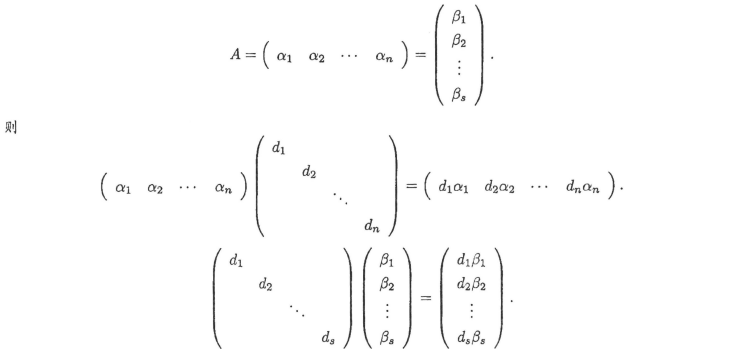
\includegraphics[scale=0.6]{6.png}
	\end{figure}
	
	即$A$右乘对角矩阵$\textup{diag}(d_1,d_2,\dots,d_n)$相当于给$A$的第$i$列元素都乘以$d_i$,
	$A$左乘对角矩阵$\textup{diag}(d_1,d_2,\dots,d_n)$相当于给$A$的第$i$行元素都乘以$d_i$。
\end{theorem}
\begin{theorem}
	(请自行完成以下内容的补充)

	对角矩阵以及准对角矩阵的三则运算、可逆性以及逆运算、乘方运算等规则。
\end{theorem}

\subsubsection{上(下)三角矩阵}
\begin{theorem}
	已知$A$,$B$都是上三角矩阵,且设$A$的主对角元素分别为$a_{11},\dots,a_{nn}$,B的主对角元素分别为
	$b_{11},\dots,b_{nn}$,则
	
	\textup{(1)}$A^{\mathrm{T}}$,$B^\mathrm{T}$都是下三角矩阵;
	
	\textup{(2)}$AB$仍然是上三角矩阵,且$AB$的主对角元素为$a_{11}b_{11},\dots,a_{nn}b_{nn}$;
	
	\textup{(3)}$A$可逆的充要条件是其主对角元均不为$0$,且$A$可逆时,$A^{-1}$也是上三角矩阵,并且$A^{-1}$的主对角元素分别为$a_{11}^{-1},\dots,a_{nn}^{-1}$.
\end{theorem}

\begin{example}
	已知$A_1,\dots,A_n$是$n$个对角元都为$0$的上三角矩阵,证明:$A_1A_2\dots A_n=O$.
\end{example}

\subsubsection{基本矩阵}
只有一个元素为1,其余元素全为0的矩阵称为基本矩阵,第$i$行第$j$列元素为1的基本矩阵记为$E_{ij}$,
他们具有如下性质(可以回忆左右乘对应行列变换):
\begin{theorem}

	\textup{(1)}$AE_{ij}$的结果就是把$A$的第$i$列移到第$j$列的位置,其余元素都为$0$的矩阵;
	
	\textup{(2)}$E_{ij}B$的结果就是把$B$的第$j$行移到第$i$行的位置,其余元素都为$0$的矩阵;
	
	\textup{(3)}$E_{ik}E_{kj}=E_{ij}$,当$k \neq l$时,有$E_{ik}E_{lj}=O$.
\end{theorem}

\subsubsection{其他矩阵}
其他矩阵如正交矩阵、置换矩阵、幂等矩阵、幂零矩阵等,有的会在稍后介绍部分性质,有的
则会在课程进行中或者后续课程中再见到它们。

\subsection{逆矩阵的求解(进阶方法)}
\subsubsection{给定多项式求逆矩阵}
此类题目相信大家已经有所见识,实际上就是通过一些初中所学的因式分解等基本变换得到需要求逆的矩阵与另一个矩阵相乘
可以得到单位矩阵(的一个倍数)。
\begin{example}
	设$A$为非零矩阵,且$A^3=O$,证明:$E+A$和$E-A$都可逆.
\end{example}

\begin{example}
	若$X$,$Y$是两个列向量,且$X^\mathrm{T}Y=2$,证明:

	\textup{(1)}$(XY^\mathrm{T})^k=2^{k-1}(XY^{\mathrm{T}})$;

	\textup{(2)}如果$A=E+XY^\mathrm{T}$,则$A$可逆,并求其逆矩阵.

\end{example}

\subsubsection{利用分块矩阵初等变换*}
我们在前面已经讲解过了打洞法的基础题型,这里再给出一些例子:
\begin{example}
	设$A$、$B$为$n$阶矩阵,证明:若$E\pm AB$可逆,则$E\pm BA$可逆.
\end{example}
\begin{example}
	设$A$为$n$阶矩阵,$B$、$C$分别为$n \times m$、$m \times n$阶矩阵,
	证明:$E_m+CA^{-1}B$可逆$\iff A+BC$可逆.
\end{example}

\subsubsection{求逆的分式思想*}
虽然矩阵没有除法运算,但是我们如果将$(E-A)^{-1}$写成$\frac{E}{E-A}$,再类比泰勒展开
$$\frac{1}{1-x}=1+\sum_{n=1}^\infty x^n(x\in (-1,1))$$我们可以得到(不严谨!只能用来解题的时候当作初步的思路!)
$$(E-A)^{-1}=\frac{E}{E-A}=E+A+A^2+\dots$$

\begin{example}
	已知方阵$A$满足$A^k=O$,其中$k$是一个正整数,求$E-A$的逆.
\end{example}

\begin{example}
	设$A$,$B$分别是$n \times m$和$m \times n$的矩阵,且$E_n \pm AB$可逆,则$E_m \pm BA$可逆.
\end{example}
不难发现这一例是前述4.3.1节中最后一个例题的推广。

\subsubsection{提逆思想*}
这一思想的来源是矩阵逆没有加减相关的运算法则,因此我们需要提逆产生一些乘积项来解决问题。
\begin{example}
	设$A$是$n$阶方阵,且$E-A$,$E+A$和$A$都可逆,证明:$(E-A^{-1})^{-1}+(E-A)^{-1}=E$.
\end{example}

\subsection{矩阵的迹*}
\subsubsection{基本概念与性质}
\begin{definition}
	一个方阵$A$的所有主对角元素之和称为$A$的迹,记为$\textup{tr}(A)$.
\end{definition}
迹的常见性质如下:
\begin{theorem}
	已知$A$,$B$是两个$n$阶矩阵,$k$是一个常数,则

	\textup{(1)}\textup{tr}$(kA)$=$k$\textup{tr}$(A)$;

	\textup{(2)}\textup{tr}$(A+B)$=\textup{tr}$(A)+$\textup{tr}$(B)$;
	
	\textup{(3)}\textup{tr}$(AB)$=\textup{tr}$(BA)$;
	
	\textup{(4)}如果$A$是实矩阵,则$A=O \iff$\textup{tr}$(A^{\mathrm{T}}A)=0$.
\end{theorem}

我们先来看一个基本的例子练习一下:
\begin{example}
	证明:不存在方阵$A$、$B$使得$AB-BA=E$.
\end{example}

接下来我们介绍一个性质,这一性质的证明需要利用矩阵的秩中讲到的一些技巧:
\begin{theorem}
	已知 $n$ 阶矩阵 $A$ 的秩为 $1$ ,证明:$A^k=\textup{tr}(A)^{k-1}A$.
\end{theorem}
这一定理的证明需要用到矩阵的分解,在2020年吴志祥老师班期中考试有出现,可以参考
辅学网站上的解答。

当然我们还会在特征值一章再次见到矩阵的迹,相关内容在最后一个专题会展开讲述。

\subsubsection{幂零矩阵}
幂零矩阵是一种特殊的矩阵,幂零矩阵$A$存在一个正整数$k$使得$A^k=O$,
它具有如下性质(部分需要用到特征值,所以最后一个专题还会提及):
\begin{theorem}
	若$n$阶矩阵$A$为幂零矩阵,则

	\textup{(1)}$A^n=O$;

	\textup{(2)}$A\pm E$均为可逆矩阵;

	\textup{(3)}幂零矩阵对应的线性变换一定存在一个矩阵表示使得矩阵为上三角矩阵且对角线元素全为\textup{0};
	
	\textup{(4)}$A$为幂零矩阵$\iff \forall k \in N^+$,\textup{tr}$(A^k)$=\textup{0}.
\end{theorem}

\begin{example}
	若$A$、$B$为两个$n$阶矩阵且满足$AB-BA=A$,证明:

	\textup{(1)}$A$不可逆;

	\textup{(2)}$A$是幂零矩阵.
\end{example}

\subsection{矩阵的幂}
\begin{enumerate}
	\item 找规律
	
	在矩阵的转置中我们已经见识了一种找规律的方式,下面是一种类似的题型:
	\begin{example}
		计算$(PAQ)^k$,其中
		$$P=\begin{pmatrix}2 & 3 \\ 1 & 2\end{pmatrix}, A=\begin{pmatrix}2 & 0 \\ 0 & -1\end{pmatrix}, Q=\begin{pmatrix}2 & -3 \\ -1 & 2\end{pmatrix}$$
	\end{example}
	
	\begin{example}
		设$A=\begin{pmatrix}0 & -1 & 0 \\ 1 & 0 & 0 \\ 0 & 0 & -1 \end{pmatrix}$,
		$P^{-1}AP=B$,求$B^{2004}-2A^2$.
	\end{example}

	还有一种找规律基于幂等矩阵,显然幂等矩阵的任意次方都与其平方相等是很好的性质,另一种找规律基于对合矩阵,即平方等于单位矩阵的矩阵,我们这里
	主要与大家分享关于幂零矩阵的方法,例子如下:
	\begin{example}
		求$A=\begin{pmatrix}a & 1 & 0 & 0 \\ 0 & a & 1 & 0 \\ 0 & 0 & a & 0 \\ 0 & 0 & 0 & a \end{pmatrix}^n$.
	\end{example}
	在上例中,我们采用将矩阵分为$A=tE+B$的方法,会发现矩阵$B$为上三角矩阵且对角线上全为0,是典型的幂零矩阵,利用这一性质可以快速解题。
	\item 数学归纳法
	\begin{example}
		求$A=\begin{pmatrix}\cos\alpha & \sin\alpha \\ -\sin\alpha & \cos\alpha\end{pmatrix}^n$.
	\end{example}
	这一问题对应我们常见的旋转变换。
	\begin{example}
		证明$\begin{pmatrix}
			a & c \\ 0 & b
		\end{pmatrix}^n=\begin{pmatrix}
			a^n & (a^{n-1}+a^{n-2}b+\dots+b^{n-1})c \\ 0 & b^n
		\end{pmatrix}$.
	\end{example}
	\item 利用秩为1的矩阵
	
	在我们有关秩的讨论中已经提到了如果$A$是秩为1的矩阵,那么$A^n=(\textup{tr}(A))^{n-1}A$,我们可以利用这一性质解决问题。
	\begin{example}
		已知$M$是秩为$1$的矩阵,记\textup{tr}$(M)=b$,讨论$(aE+M)^n$的计算结果.
	\end{example}

	\begin{example}
		已知$A$是数域$P$上的一个$2$阶方阵,且存在正整数$l$使得$A^l=O$,证明:$A^2=O$.
	\end{example}
	事实上,我们在幂零矩阵的讨论中已经提及了上例的一般情况。

	\begin{example}
		已知数列$\{a_n\}$,$\{b_n\}$满足$a_0=-1$,$b_0=3$,且
		$$\begin{cases}
			a_n=3a_{n-1}+b_{n-1}+2^{n-1} \\ b_n=2a_{n-1}+4b_{n-1}+2^n
		\end{cases}$$
		求$\{a_n\}$,$\{b_n\}$的通项公式.
	\end{example}
	\item 利用初等矩阵的性质
	\begin{example}
		设$A$为三阶矩阵,$P$为三阶可逆矩阵,$P^{-1}AP=B$,其中$P=\begin{pmatrix}
			0 & 2 & -1 \\ 1 & 1 & 2 \\ -1 & -1 & -1
		\end{pmatrix}$,$B=\begin{pmatrix}
			0 & 0 & -1 \\ 0 & -1 & 0 \\ -1 & 0 & 0
		\end{pmatrix}$,求$A^{2022}$.
	\end{example}

	\item 利用对角化
	
	若一个矩阵$A$可对角化,即存在可逆矩阵$P$使得$A=P^{-1}\Lambda P$(其中$\Lambda$为对角矩阵),
	在这种形式下$A$的幂是很好求的。
	\begin{example}
		已知$A=\begin{pmatrix}
			0 & \cfrac{1}{2} & \cfrac{1}{2} \\ 1 & -\cfrac{1}{2} & \cfrac{1}{2} \\ 1 & -\cfrac{1}{2} & \cfrac{1}{2}
		\end{pmatrix}$,求$A^n$.
	\end{example}

\end{enumerate}

\section{矩阵的秩的定义与性质}
本节内容理解难度较大,事实上这里利用了很多线性空间与线性映射的思想,
也有很多技巧性的内容,因此希望各位同学根据自己实际情况理解掌握。虽然很推荐
这部分内容采用与教材不同的思路去理解,更多利用线性空间与线性映射的抽象知识思考,但是如果
理解起来有一定困难也记住一些结论去解决一些问题。

还有一部分应当属于本节的内容将在专题五线性方程组的部分提及,因此本节不再专门
讲解利用线性方程组的思想解决矩阵的秩相关问题的部分。

\subsection{矩阵的三个秩的基本概念与性质}
我们首先给出矩阵的三个秩的定义:
\begin{definition}
	设$A$是线性映射$\sigma$对应的矩阵,我们把$\sigma$的秩也称为矩阵$A$的秩,
	记为$r(A)$.我们将矩阵$A$的所有行向量组成的秩称为$A$的行秩,
	所有列向量组成的向量组的秩称为$A$的列秩.
\end{definition}
对于以上三个秩我们有重要的定理如下:
\begin{theorem}
	任意矩阵的秩 = 行秩 = 列秩.
\end{theorem}
这一定理的证明,矩阵的秩 = 列秩的部分根据线性映射的相关概念是显然的,行秩的部分
教材中有较为繁琐的证明,在本讲义下面的内容会有更加形象的解释。

实际上,这一定理有两个重要的直接推论,一是将求矩阵的秩的问题转化为求矩阵行/列极大线性无关向量组的问题,
第二是矩阵的秩等于其转置的秩。

可能很多同学对于行秩、列秩相等以及转置的几何意义很感兴趣。实际上我们有两种获得转置矩阵的
方式,第一种来源于我们之前讨论的对偶空间上的线性映射对应的矩阵,这种方式可能不够直观。
另一种获得的方法基于内积,感兴趣的同学可以了解矩阵的伴随(不是行列式中的伴随矩阵)。

我们可以研究矩阵及其转置的关系,我们可以用一个图形来表示:
\begin{figure}[h]
	\centering
	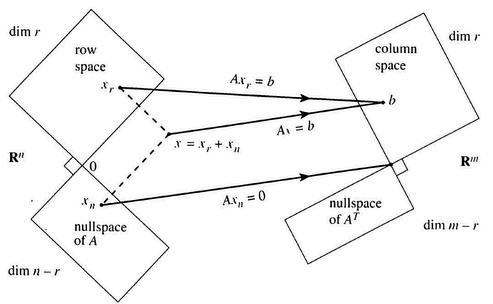
\includegraphics[scale=0.5]{5.png}
\end{figure}

我们观察到以下几点:
\begin{enumerate}
	\item 矩阵的行空间与解空间(零空间)互为正交补(直观理解两个空间就是互相垂直且互为补空间),这一点应当是在正交的内容中有所提及的;
	\item 矩阵的列空间与其转置矩阵的零空间互为正交补,这一点实际与上一条等价.
\end{enumerate}

接下来我们来看行秩(列秩比较显然,此处不再详细展开)。我们首先得到解空间的维数,这可以直接
根据维数公式得到:$\dim N(A)=n-r(A)$,根据正交补的性质,我们的可以得到行秩即为
$n-(n-r(A))=r(A)$.于是我们得到了一个基于正交补的行秩解释.

\subsection{相抵标准形}
此处我们需要首先回顾一个基本定理:
\begin{theorem}
	初等变换不改变矩阵的秩(包括行变换和列变换).
\end{theorem}
由这一定理我们可以推导出相抵标准形:
\begin{theorem}
	若$r(A_{m \times n})=r$,则存在可逆矩阵$P$和$Q$,使得
	$$PAQ=\begin{pmatrix}
		E_r & 0 \\ 0 & 0
	\end{pmatrix}=U_r,$$
	其中$E_r$表示$r$阶单位矩阵.
\end{theorem}
这一定理证明直接使用定理4以及可逆矩阵可以拆分为初等矩阵的乘积即可。
其中$U_r$称为相抵标准形。我们称两个矩阵相抵即两个矩阵可以通过一系列
初等变换可以互相转化。由此我们得到关于矩阵相抵的两个等价命题:

1. 矩阵$A$与$B$相抵$\iff$存在可逆矩阵$P$和$Q$使得$PAQ=B$;

2. 矩阵$A$与$B$相抵$\iff r(A)=r(B)$.

\begin{example}
	设$A=\begin{pmatrix}
		1 & 0 & 2 & -4 \\ 2 & 1 & 3 & -6 \\ -1 & -1 & -1 & 2
	\end{pmatrix}$, 求

	\textup{(1)}$A$的秩$r$和相抵标准形;

	\textup{(2)}$3$阶可逆矩阵$P$和$4$阶可逆矩阵$Q$使得$PAQ=\begin{pmatrix}
		E_r & 0 \\ 0 & 0
	\end{pmatrix}$.
\end{example}

关于相抵标准形,我们需要在此补充一个常用的技术,即相抵标准形的分解:

我们对$s \times n$矩阵$\begin{pmatrix}
	E_r & O \\ O & O
\end{pmatrix}$有一种很重要的分解:
$$\begin{pmatrix}
	E_r & O \\ O & O
\end{pmatrix}=\begin{pmatrix}
	E_r \\ O
\end{pmatrix}\begin{pmatrix}
	E_r & O
\end{pmatrix}$$ 由此我们可以知道任意一个非零矩阵都可以被分解成一个列满秩矩阵和一个
行满秩矩阵的乘积:

$$A=P\begin{pmatrix}
	E_r & O \\ O & O
\end{pmatrix}Q=P\begin{pmatrix}
	E_r \\ O
\end{pmatrix}\begin{pmatrix}
	E_r & O
\end{pmatrix}Q$$
记$P_1=P\begin{pmatrix}
	E_r \\ O
\end{pmatrix}$,$Q_1=\begin{pmatrix}
	E_r & O
\end{pmatrix}Q$,则$A=P_1Q_1$,且$P_1$和$Q_1$分别为列满秩、行满秩矩阵。

我们可以利用相抵标准形解决很多问题,例如下一节中部分秩不等式的证明:
\begin{example}
	\textup{(1)}$r\begin{pmatrix}
		A & O \\ O & B
	\end{pmatrix}=r(A)+r(B)$.

	\textup{(2)}$r\begin{pmatrix}
		A & D \\ O & B
	\end{pmatrix}\ge r(A)+r(B)$,
	$r\begin{pmatrix}
		A & O \\ C & B
	\end{pmatrix}\ge r(A)+r(B)$.
\end{example}

\subsection{秩相关的等式与不等式}
本节的内容实际上部分内容有一定的技巧性,对于荣誉课程来说还是以理解为主(所以
其实本节中提到的很多内容都只是介绍性的,而非要求大家熟练掌握,但是遇见了要有
一些基本的思路而不能完全不理解),可能下面列出定理的时候显得比较繁冗,但是实
际上我们更重视其中的理解而非硬套结论。

我们首先给出一些常见的秩相关的不等式或等式,这些式子希望各位同学能够理解其含义,
而非机械记忆套用。下面这些等式/不等式的证明方式非常多,实际上可以利用之前所说化为
相抵标准形的方法,也可以利用线性相关性的方法,也可以回到线性映射进行考量。总之
解决的方法非常多,希望各位同学能熟练推导理解。
\begin{enumerate}
	\item $r(A)=r(PA)=r(AQ)=r(PAQ)$,其中$P$、$Q$可逆
	\item $|r(A)-r(B)|\le r(A\pm B) \le r(A)+r(B)$
	\item $r(AB) \le \min\{r(A),\ r(B)\}$
	\item $r(A)=r(A^\mathrm{T})=r(AA^\mathrm{T})=r(A^\mathrm{T}A)$(注意第二个等号需要实矩阵作为前提条件)
	\item $A \in \mathbf{F}^{s \times n}$,$B \in \mathbf{F}^{n \times m}$,
	则$r(AB) \ge r(A)+r(B)-n$.(可以视为结论6的推论,特例$AB=O$时有$r(A)+r(B)\le n$)
	\item $r(ABC) \ge r(AB)+r(BC)-r(B)$.(还可以考虑A,B,C相等的特殊情况的结果)
\end{enumerate}

分块矩阵的相关公式在上一小节的例题中已经书写过,此处不再重复。

一般而言,解决较为复杂的秩的问题时,我们可以采用如下方法:

(1)利用(分块)矩阵初等变换;

(2)利用线性方程组解的一般理论(将在专题五讲解);

(3)利用向量组线性相关性;

(4)利用已知的矩阵秩的等式和不等式。实际上等式很多时候基于可逆矩阵变换或者两个不等号夹逼。

相关方法的应用都在本节最后的习题中有所体现,当然首要的任务是掌握上述基本的秩不等式的证明,
很多也利用了上面的思想,并且解法不唯一。

\subsection{习题}
\centerline{\heiti A组}
\begin{enumerate}
	\item 证明:矩阵添加一列(或一行),其秩或不变,或增加1.
	\item 设$A$是$s \times n$矩阵,$B$是$A$前$m$行构成的$m \times n$矩阵,证明:
	$r(B) \ge r(A) + m - s$.
	\item 若$A$、$B$为两个$n$阶矩阵,则

	$\textup{A}.\ r(A\ B)=r(A^\mathrm{T}\ B^\mathrm{T})$

	$\textup{B}.\ r(A\ AB)=r(A)$

	$\textup{C}.\ r(A\ B)=\max\{r(A),\ r(B)\}$

	$\textup{D}.\ r(A\ BA)=r(A)$
	\item 若$A$、$B$为两个$n$阶矩阵且满足$A+B=AB$,证明:

	(1)$A-E$和$B-E$均可逆;

	(2)$AB=BA$;

	(3)$r(A)=r(B)$.
\end{enumerate}
\centerline{\heiti B组}
\begin{enumerate}
	\item 设$A$为$n$阶矩阵,且$r(A) < n$,又$A_{11} \neq 0$,证明:存在常数$k$,使得
	$(A^*)^2=kA^*$.
	\item (利用相抵标准形)证明以下结论:
	
	(1)设$B_1$,$B_2$为$s \times n$列满秩矩阵,证明:存在$s$阶可逆矩阵
	$C$使得$B_2=CB_1$.

	(2)设$B_1$,$B_2$为$s \times n$行满秩矩阵,证明:存在$n$阶可逆矩阵
	$C$使得$B_2=B_1C$.
	
	(3)任意秩为$r$的矩阵都可以被分解为$r$个秩为$1$的矩阵之和.

	(4)已知$A$是$n$阶方阵,证明:存在$n$阶方阵$B$使得$A=ABA$,$B=BAB$.
	\item 设$B$是$3 \times 1$矩阵,$C$是$1 \times 3$矩阵,证明:$r(BC) \le 1$.
	反之,若$A$是秩为1的$3 \times 3$矩阵,证明:存在$3 \times 1$矩阵$B$和$1 \times 3$矩阵$C$,使得$A = BC$.
	\item 设$\alpha$、$\beta$为$n$维列向量,且$A=\alpha\alpha^\mathrm{T}+\beta\beta^\mathrm{T}$.
	
	(1)证明:$r(A) \le 2$;

	(2)若$\alpha$、$\beta$线性相关,证明:$r(A) \le 1$.
	\item 设 $A \in M_{m \times n}(\mathbf{F})$,$r(A)=r$,$k$ 是满足条件 $r \leq k \leq n$ 的任意整数,证明存在 $n$ 阶方阵 $B$,使得 $AB=O$,且 $r(A)+r(B)=k$.
	\item 设$A$是$m \times n$矩阵($m \le n$),$r(A)=m$,证明:存在$n \times m$矩阵$B$使得$AB=E$.
	\item 设$A,\ B \in M_n(\mathbf{F})$,$r(A)+r(B) \le n$,证明:存在可逆矩阵$M$,使得$AMB=O$.
\end{enumerate}

\centerline{\heiti C组}
\begin{enumerate}
	\item (打洞法)已知$A$是一个$s \times n$矩阵,证明:$r(E_n-A^\mathrm{T}A)-r(E_s-AA^\mathrm{T})=n-s$.
	\item 利用打洞法完成以下两个问题((2)也可以不使用打洞法,可以思考其他方式解决):
	
	(1)设$n$阶方阵$A$,$B$,$C$,$D$满足$AC+BD=E$,证明:$r(AB) = r(A)+r(B)-n$.
	
	(2)$n$阶方阵$A$,$B$满足$AB=BA$,证明:$r(AB)+r(A+B)\le r(A)+r(B)$.
	\item $f(x)=f_1(x)f_2(x)$是多项式,且$f_1(x)$与$f_2(x)$互素,则$f(A)=O$的充要条件是$r(f_1(A))+r(f_2(A))=n$.
	(注:此题的推论非常多,如$A^2=A$,$A^n=E$等形式的结论都可以利用这个例子推导出)
	\item 设$A$、$B$分别为$3 \times 2$和$2 \times 3$实矩阵,若$AB=\begin{pmatrix}
		8 & 0 & -4 \\ -\cfrac{3}{2} & 9 & -6 \\ -2 & 0 & 1
	\end{pmatrix}$,求$BA$.
\end{enumerate}
